Task B7 was to implement video driver functions so that the kprinthex and kprints methods in the kernel were replaced, so that text was printed to the VGA screen, instead of the bochs console. Also we needed to implement a system call, printat, so that running programs have the option to print to any column/row. When writing to a specific memory position (0xB8000 in bochs) you are essentially writing to the ``text mode'' area of the video hardware. This mode allows us to directly and simply write characters onto a predefined screen configuration. On bochs it is defined as a screen with 80x24 (1920) characters. Then all that is needed is to write a driver that is able to handle the syntax and data that the hardware receives and returns. A common way of communicating with hardware is to map some, in advance, agreed upon location in the computer's memory to input/output signal of another hardware component, which the software and hardware is able to communicate though.\
\\\
In our case of a video driver, if we imaging that figure~\ref{fig:display} is a whole screen with very bad resolution or pixel/tile density, where characters can only be placed in those limited boxes. On the figure~\ref{fig:display} screen there could only be a maximum of 16 (rows multiplied by columns) characters. – The course book\cite{TanenbaumWoodhull08} has a screen represented by 24 rows and 80 columns, but that would make for too big example.
\subsection{Implementation}

\begin{figure}
\centering
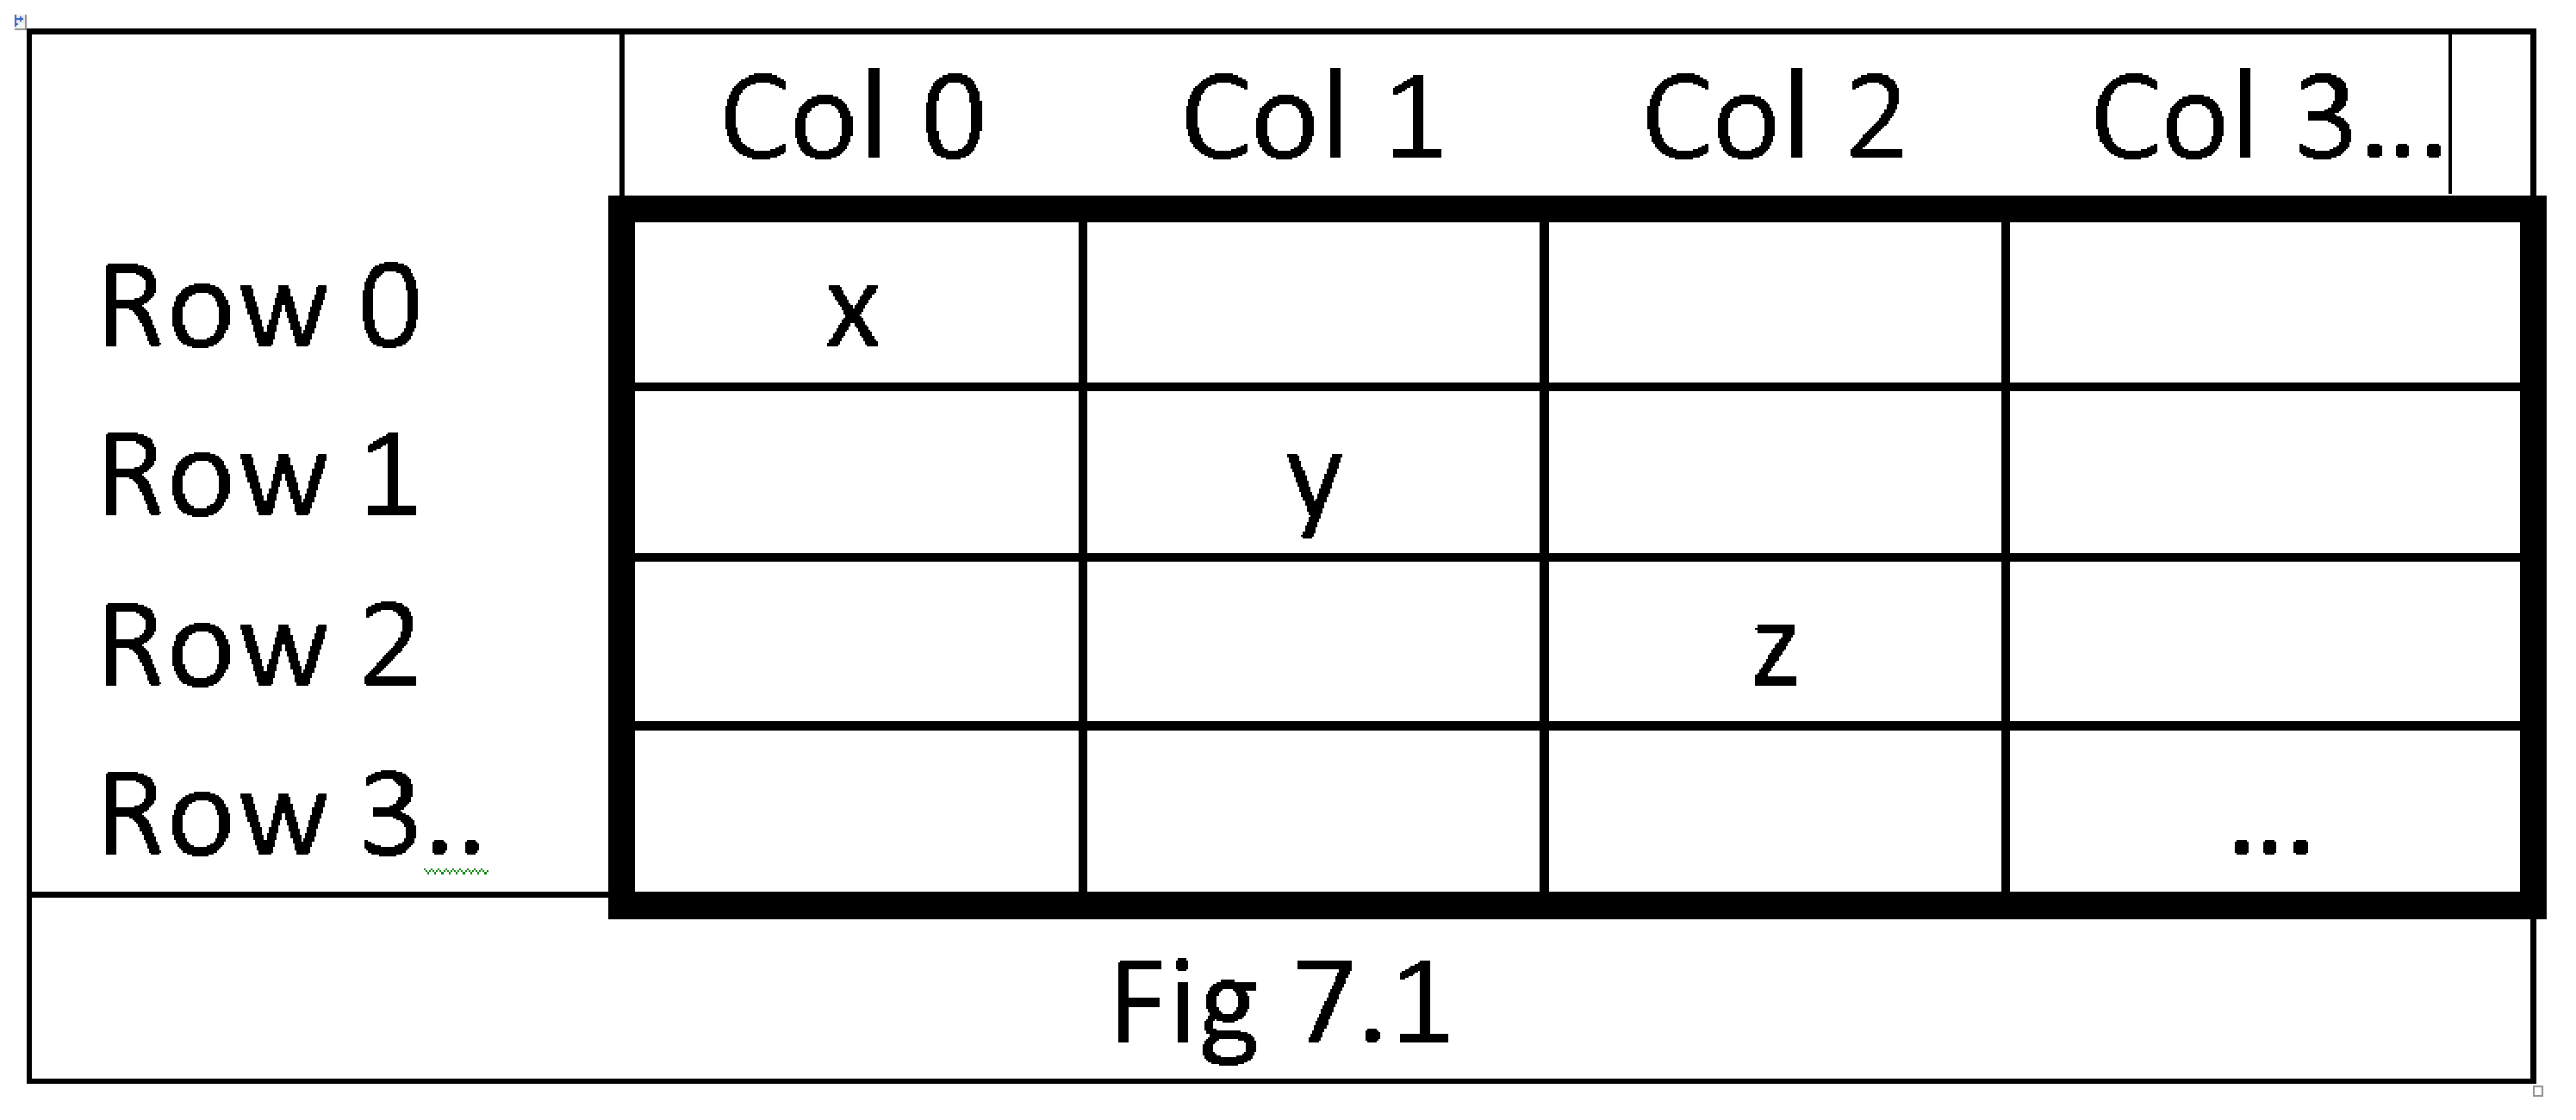
\epsfig{file=fig/Display.eps, height=1in}
\caption{The VGA display}
\label{fig:display}
\end{figure}


\subsubsection*{video.c}


The video driver is very basic and does not implement scrolling of text. For our implementation of the kprints and kprinthex we made a supplemental method call print\_char which simply sets the char for a given x, y coordinate. \\\\
What we essentially reply on is to loop though all the input text for our kprints so that it uses the print\_char with the current row we are on, while incrementing your current column so we print. As we loop through the characters of our string, we check for certain conditions. If the current row is equal to the predefined maximum row then we just set the current row to 0, so that the text simply continues from the top, or wraps around. Also if the conditions are met for either a newline character or we have reached the last column, then we increment the current row by one, and set the current column to 0.
When we need the kprinthex method we can rely on our kprints method to handle all the logic and parsing. All that is needed is to convert our hexadecimal input number into a string, and then send this string to the kprints method.
The syscall “printat” is very similar to kprints in regards to behavior, except the printat takes the initial row and column as arguments, so these are transferred via the rsi and rdi registers.
 The code is very simple and easily read - please see the project file “video.c” and “syscall.c” for further details.

\subsection{Reflections}

\subsubsection*{How would you implement support for scrolling?}
A possibility would be to have some code that would overwrite every column into the row above its immediate position.  That means that on the imaginary screen of figure~\ref{fig:display} the row 1, column 0 would be copied to row 0, column 0. This would be done with all the rows, and the ``illusion'' of scrolling would appear, and the last available row would be free to write into. Since we would be overwriting/destroying all the values in row 0, this might not be the most elegant scrolling solution, but is relatively simple and memory conserving, if not light on the CPU.\\
\\
Another solution might involve manipulation of the video pointer. A linked list could be used containing all the individual rows, with in turn contain all the columns for the individual rows. So instead of changing all the values in the rows, the linked list order is manipulated. So that if the end of the screen is reached, then the first row to display is changed from row 0 to row 1 for example. Then the last row will go from row 3 to row 0, and row 0 is cleared of values. This is a little more complicated solution, but would be more CPU load efficient compared to the previous solution. Since the video hardware reads data directly from memory, a linked list might not be technically compatible.\\
\\
The course lecture book explains another way of implementing a scrolling function, and uses a register which the video hardware is able to read, so that it has a start location for reading its input. This way we only need to increment the start location for each line as needed, and no large operations copying/moving of data are needed, since the video hardware is controlling in which order data is read, thereby lowering CPU load.
	